% "{'classe':('PSI'),'chapitre':'tec_','type':('td'),'titre':'Système de dépose de poudre', 'source':'Concours Centrale Supelec -- TSI 2016','comp':('C1-05','C2-08'),'corrige':False}"
%\setchapterimage{bandeau}
\chapter*{TD \arabic{cptTD} \\ 
Système de dépose de poudre -- \ifprof Corrigé \else Sujet \fi}
\addcontentsline{toc}{section}{TD \arabic{cptTD} : Système de dépose de poudre -- \ifprof Corrigé \else Sujet \fi}

\iflivret \stepcounter{cptTD} \else
\ifprof  \stepcounter{cptTD} \else \fi
\fi

\setcounter{question}{0}
\marginnote{Concours Centrale Supelec -- TSI 2016}
\marginnote[1cm]{
\UPSTIcompetence[2]{C1-05}
\UPSTIcompetence[2]{C2-08}}


\begin{marginfigure} [4cm]
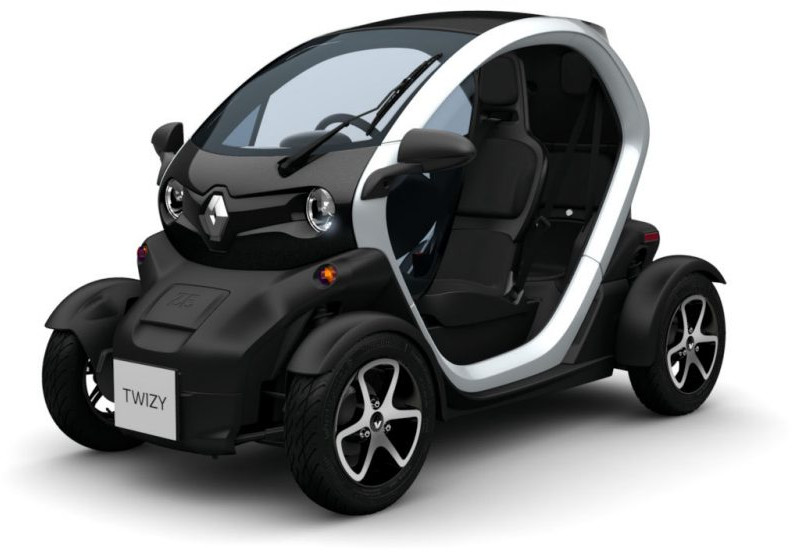
\includegraphics[width=\linewidth]{fig_01}
\end{marginfigure}




\section*{Mise en situation}
\ifprof
\else
On s'intéresse à un système permettant de créer des motifs sur de la poudre de maquillage compactée. Le poste de pulvérisation est en partie constitué d'un robot cartésien 3 axes permettant de déplacer des godets de poudre compactée (grâce à un préhenseur) en dessous de la buse de pulvérisation. 

\begin{center}
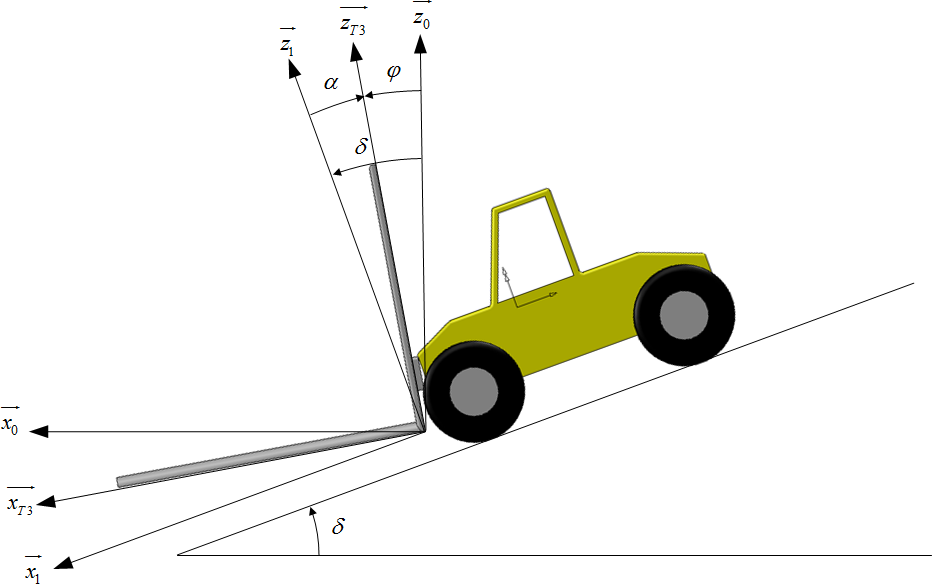
\includegraphics[width=.7\linewidth]{fig_02}
\end{center}

\fi

\begin{obj}
L’objectif est de valider le choix du moteur effectué par le concepteur du système.

Le cahier des charges impose que la vitesse maximale du chariot sur l’axe $\vect{x}$ soit de $V_{\text{max}}= \SI{0,45}{m.s^{-1}}$ et que l’accélération maximale du chariot soit de $\gamma_{\text{max}}= \SI{10}{m.s^{-2}}$.
\end{obj}

\subsection*{Travail demandé}

\ifprof
\else
La transmission est réalisée de la façon suivante. L'arbre 1 est entrainé par un moto-réducteur dont le raport de réduction est noté $r$. 

\begin{marginfigure}
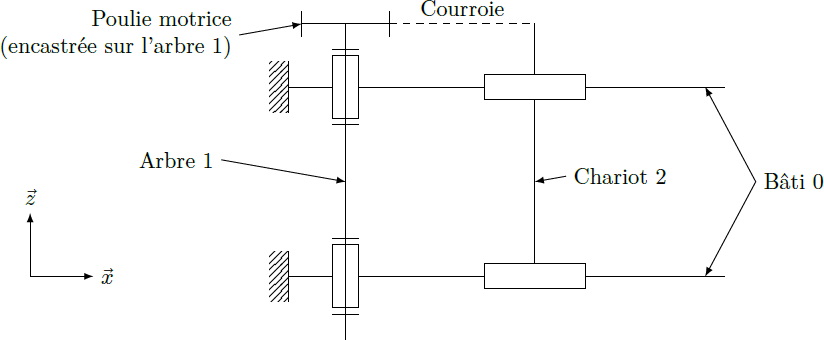
\includegraphics[width=\linewidth]{fig_05}
\end{marginfigure}

\noindent\textbf{Notations}
\begin{itemize}
\item $\Omega$ : vitesse de rotation du moteur;
\item $C_m$ : le couple exercé par le moteur;
\item $r=n_{\text{axe poulie}}/n_{\text{moteur}}=\dfrac{1}{10}$: rapport de réduction du réducteur entre le moteur et les poulies;
\item $M_2 = \SI{25}{kg}$ : masse de l’ensemble mobile 2;
\item $\phi = \SI{28,65}{mm}$ est le diamètre primitif des poulies;
\item l’inertie des courroies est négligée;
\item $J_m = \SI{1,2e-5}{kg.m^2}$ : moment d’inertie de l’arbre moteur;
\item $J_1 = \SI{4e-4}{kg.m^2}$ : moment d’inertie de l’arbre 1;
\item $C_r = \SI{0,15}{Nm}$ : couple de frottements secs dans les liaisons ramené à l’arbre moteur;
\item $\mu = \SI{0,001}{N.m.s.rad^{-1}}$ : coefficient de frottements visqueux dans les liaisons ramené à l’arbre moteur.
\end{itemize}
\fi

\question{Déterminer la vitesse maximale de rotation du moteur $\Omega_{\text{max}}$. Faire l’application numérique.}
\ifprof
\begin{corrige}~\\
On a $V_{\text{max}}=\Omega_{\text{max}}\cdot r \cdot \dfrac{\phi}{2}$. En conséquence 
$\Omega_{\text{max}}=V_{\text{max}}\dfrac{2}{r \phi}$. 

\textit{Application numérique :} $\Omega_{\text{max}}=\dfrac{2\cdot 0,45 \cdot 10}{28,65\times 10^{-3}}\simeq\SI{314}{rad.s^{-1}}\simeq\SI{3000}{tr.min^{-1}}$.

\end{corrige}
\else
\fi

\question{Déterminer l’accélération maximale du moteur $\dot{\Omega}_{\text{max}}$. Faire l’application numérique.}
\ifprof
\begin{corrige}~\\
En suivant un raisonnement similaire : 
$\dot{\Omega}_{\text{max}}=\gamma_{\text{max}}\dfrac{2}{r \phi}$. 


\textit{Application numérique : } $\dot{\Omega}_{\text{max}}=\dfrac{10\cdot 2\cdot 10}{ 28,65\times 10^{-3}}\simeq \SI{6981}{rad.s^{-2}}$. 


\end{corrige}
\else
\fi


\question{Donner l’expression de l’énergie cinétique de l’ensemble mobile dans son mouvement le long de l’axe $\vect{x}$ par rapport au bâti notée $\mathcal{E}_c\left(\text{ensemble}/0\right)$. En déduire l’inertie équivalente $J$ de l’ensemble mobile rapportée à l’arbre du moteur. Faire l’application numérique.}
\ifprof
\begin{corrige}~\\
Le système peut être modélisé ainsi :

\begin{center}
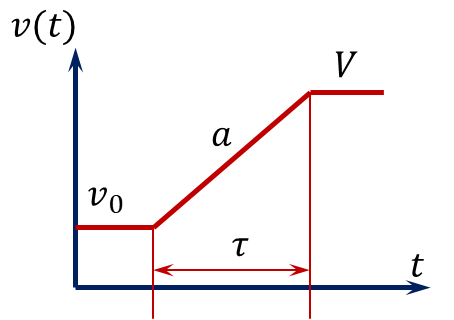
\includegraphics[width=.7\linewidth]{cor_01}
\end{center}

$\mathcal{E}_c\left(\text{ensemble}/0\right) = \mathcal{E}_c\left(1/0\right)+\mathcal{E}_c\left(2/0\right)$. Le solide 1 et l'arbre moteur sont en rotation par rapport au bâti et le solide 2 est en translation par rapport au bâti, on a donc : 
\begin{itemize}
\item $\mathcal{E}_c\left(1/0\right) = \dfrac{1}{2}\left( J_m \Omega^2 + J_1 \left(r\Omega\right)^2\right)= \dfrac{1}{2}\left( J_m  + J_1 r^2\right)\Omega^2$
\item $\mathcal{E}_c\left(2/0\right) = \dfrac{1}{2} M V^2 = \dfrac{1}{2} M \Omega^2  \left(\dfrac{r\phi}{2}\right)^2$.
\end{itemize}

$\mathcal{E}_c\left(\text{ensemble}/0\right) = \dfrac{1}{2}\left(\left( J_m  + J_1 r^2\right)+   M \left(\dfrac{r\phi}{2}\right)^2\right)\Omega^2  $.


\textit{Application numérique : }
$J_{eq}=\left( J_m  + J_1 r^2\right)+   M \left(\dfrac{r\phi}{2}\right)^2 =5,9\times 10^{-5} \, \text{kg m}^2$.
\end{corrige}
\else
\fi

\question{Établir l’expression du couple moteur maximal exercé par le moteur sur l’arbre moteur noté $C_{\text{max}}$. Faire l’application numérique.}
\ifprof
\begin{corrige}~\\
\end{corrige}
\else
\fi


\question{Donner l’expression de la puissance mécanique maximale que devra fournir le moteur électrique. Faire l’application numérique.}
\ifprof
\begin{corrige}~\\
\end{corrige}
\else
\fi

Le concepteur du système a choisi un moteur synchrone de vitesse nominale de $\SI{3000}{tr.min^{-1}}$ et de puissance utile $\SI{0,47}{kW}$.

\question{Valider le choix du moteur en le justifiant. Argumenter la présence éventuelle d’écart entre la puissance mécanique maximale calculée et la puissance nominale du moteur choisi.}
\ifprof
\begin{corrige}~\\
\end{corrige}
\else
\fi

